\chapter{Kirjautumismenetelmien vertailu\label{vertailu}}

Tässä kappaleessa vertaillaan kirjautumismenetelmiä. Kappaleessa vertaillaan kuuden valitun kirjautumismenetelmän soveltuvuutta neljässä käyttötarkoituksessa. 


Kaksi- ja monivaiheisia kirjautumistapoja on todettu olevan monia erilaisia menetelmiä. Myös käyttötarkoituksia, joissa näitä menetelmiä käytetään, on olemassa monia. Seuraavaksi vertaillaan kuutta varmentamismenetelmää neljässä eri käyttötarkoituksessa. Vertailuun ei ole valittu yksittäisiä käyttötarkoituksia kuten yksittäistä verkkosivua vaan yleisimpiä kategorioita, jotka kuvaavat laajempaa käyttötarkoitusjoukkoa. Valitut kirjautumismenetelmät sekä käyttötarkoitukset pyrkivät kuvaamaan monipuolisesti varmentamismenetelmien soveltuvuutta eri käyttötarkoituksissa. 

Vertailuun valitut varmentamismenetelmät ovat SMS-varmenne, kertakäyttöiset koodit, fyysinen avain, mobiilisovelluksella varmentaminen, sähköposti ja verkkopankkitunnukset.

Pankit vaativat nykyään verkkopankkitunnuksen lisäksi kaksivaiheisen tunnistautumisen. Kaksivaiheisia tunnistautumistapoja, joita pankit tarjoavat ovat mobiilisovellus, kertakäyttöiset koodit ja tekstiviestivahvistus \citep{nordea_tunnistautuminen} \citep{op_tunnistautuminen} \citep{spankki_tunnistautuminen}. Verkkopankkiin kirjautumisessa yhdistyy vertailun varmentamismenetelmiä. Tämä takia tutkimuksen vertailun oletuksena on, että verkkopankkitunnukseen sisältyy pankkitunnus sekä kirjautumiseen vaadittava kaksivaiheinen tunnistautuminen.

Vertailussa käytettävät käyttötarkoitukset ovat verkkosivut, pankkipalvelut, julkisetpalvelut sekä IoT-laitteet. Verkkosivuilla tarkoitetaan yleisellä tasolla verkossa olevia sivustoja, joiden käyttämiseen vaaditaan kirjautumista, jotta käyttäjä voidaan tunnistaa ja tarjota yksilöllistä sisältöä. 

Verkkopankkien käyttäminen laskujen maksamiseen on yleistynyt merkittävästi tämän vuosituhannen aikana. Nykyään noin 88\% ihmistä ja 97\% 25–44-vuotiaisista käyttää verkkopankkia maksujen maksamiseen \citep{säästäminen_luotonkäyttö_maksutavat} Verkkopankit ovat täten kriittisiä ja tärkeitä palveluita.

Julkiset palvelut ovat pankkipalveluiden tapaan tärkeitä ja kriittisiä palveluita. Suomessa julkisia palveluita ovat esimerkiksi veroasioiden hoitamiseen Omavero, terveydenhuollon Omakanta sekä opintojen ja koulutusten palvelu Opintopolku. Julkisissa palveluissa käsitellään ihmisten tärkeitä tietoja. Varmentaminen näihin palveluihin täytyy olla varma ja vahva.

IoT-laitteiden verkosto koostuu valtavasta määrästä fyysisiä laitteita. Tämän tuo erilaisia vaatimuksia sekä haasteita varmentamiseen.

Varmennusmenetelmien soveltuvuutta arvioidaan viisiportaisella asteikolla nollasta neljään. Nolla tarkoittaa, että kyseinen varmentamismenetelmä ei sovellu lainkaan käyttötarkoitukseen. Ykkönen tarkoittaa, että menetelmä sopii, mutta ei ole suositeltava. Kaksi tarkoittaa, että kyseessä on mahdollinen käytettävä varmentamismenetelmä, mutta siihen saattaa liittyä joitakin ongelmia. Arvosana kolme tarkoittaa, että varmentamismenetelmä on suositeltava vaihtoehto. Korkein arvosana neljä tarkoittaa, että varmentamismenetelmä on vahvasti suositeltava ja sitä tulisi käyttää.

Nämä käyttötilanteen on koottu tauluun \ref{tab:vertailu}. Seuraavassa arvioidaan edellä käsiteltyjä varmenteita kussakin käyttöskenaariossa.

\begin{table}[ht]
\begin{tabular}{ |p{3cm}|p{1cm}|p{1,5cm}|p{1,5cm}|p{1,5cm}|p{2cm}|p{2,5cm}|  }
 \hline
 \multicolumn{7}{|c|}{ Kirjautumismenetelmät} \\
 \hline
 & SMS & TOTP &Fyysinen avain & Mobiili-sovellus & sähköposti & Verkkopankki-tunnukset\\
 \hline
 Verkkosivut& 4 & 3 & 4 & 4 & 2 & 1\\
 Pankkipalvelut& 1 & 1 & 1 & 1 & 1 & 4\\
 Julkisetpalvelut& 1 & 1 & 1 & 1 & 1 & 4\\
 IoT-laitteet& 2 & 4 & 4 & 2 & 2 & 0\\
 \hline
 \multicolumn{7}{|c|}{
0: ei sovellu
1: ei suositeltava
2: mahdollinen
3: suositeltava
4: vahva suositus} \\
\hline

\end{tabular}
\caption{\label{tab:vertailu} Kirjautumismenetelmien vertailu}
\end{table}

Verkkosivujen käytöstä kuva \ref{fig:account_takeover_rates} havainnollistaa miten eri varmentamismenetelmät ovat estäneet automaattisia bottihyökkäyksiä, kalasteluhyökkäyksiä ja kohdennettuja hyökkäyksiä. Kuvasta \ref{fig:account_takeover_rates} nähdään, että fyysinen avain on parhainten estänyt kaikkia hyökkäyksiä. SMS-varmenne sekä mobiilisovelluksella tapahtuva kirjautuminen ovat myös estäneet paljon hyökkäyksiä. Näiden tulosten perusteella SMS-varmenne ja mobiilisovelluksella tapahtuva kirjautuminen ovat vahvasti suositeltavia. Toisen sähköpostiosoitteen käyttäminen on estänyt hyökkäyksiä, mutta vain noin 70 \%. Sähköpotin käyttäminen ei ole tuonut yhtä hyvää suojaa kuin SMS-varmenne, fyysinen avain ja mobiilisovellus. Tämän takia sähköposti on suositeltava, mutta ei vahvasti suositeltava vaihtoehto. Verkkopankkitunnuksien käyttäminen verkkosivuilla on mahdollista, mutta ei suositeltavaa. Verkkopankkitunnukset ovat tärkeitä ja kriittisiä, joten käyttäminen ei ole suositeltavaa ja tämän takia annettu verkkopankkitunnuksille arvosana 1.

\begin{figure}[ht]
    \centering
    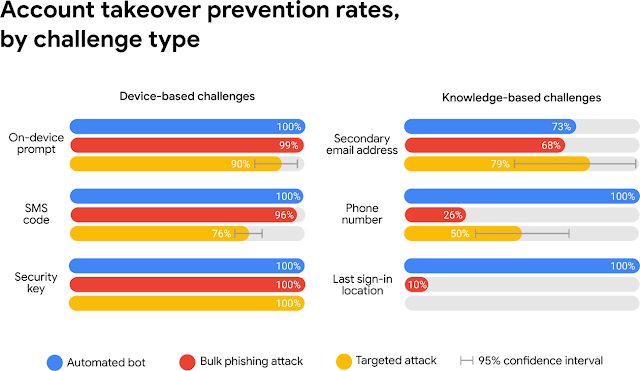
\includegraphics[width=12cm]{template/figures/account takeover provention rates.png}
    \caption{Varmentamismenetelmien tehokkuus hyökkäyksiä vastaan \citep{google_security}}
    \label{fig:account_takeover_rates}
\end{figure}

Pankkipalveluissa tärkeintä on käyttäjän henkilöllisyyden tunnistaminen ja varmentaminen. Pankkipalveluissa käsitellään raha-asioita, joka on tärkeä ja kriittinen asia. Tämän takia vain oikealla ihmisellä tulisi pelkästään olla pääsy omiin tietoihin. Tämän takia käytetään niin sanottua vahvaa tunnistautumista pankkipalveluiden kirjautumisessa \citep{kpclient}.

Suomessa pankeilla on lakisääteinen velvollisuus tunnistaa asiakkaan henkilöllisyys ennen kuin tekevät sopimuksen asiakkaan kanssa ja luovuttaa pankkitunnukset. Henkilöllisyyden todentamiseen vaaditaan virallinen henkilöllisyystodistus. Tämän pakollisen henkilöllisyyden varmentamisen avulla saadaan yhdistettyä käyttäjän pankkitunnus sekä hänen henkilöllisyytensä. Kun käyttäjä kirjautuu pankkipalveluun pankkitunnuksella, pankki pystyy yhdistämään ja varmentamaan käyttäjän henkilöllisyyden. Henkilöllisyyden varmentaminen on tärkeää koska pankkitunnusten avulla voidaan tunnistautua pankkipalveluiden lisäksi myös yksityisissä sekä viranomaisten sähköisissä palveluissa \citep{FINE_verkkopankkitunnukset}.

Pankkitunnusten vahvuus on se, että sen avulla pystytään varmentamaan käyttäjän henkilöllisyys. Täten verkkopankkitunnuksia voidaan pitää luotettava ja vahvasti suositeltavana valintana pankkipalveluissa.

Vertailun muut varmentamismenetelmät olisivat teknillisesti mahdollisia vaihtoehtoja. Mutta pankkipalveluihin kirjautuessa käyttäjän henkilöllisyyden varmentaminen on tärkeää ovat nämä menetelmät mahdollisia mutta ei suositeltavia.

Pankkipalveluiden lisäksi myös julkiset palvelut ovat tärkeitä ja kriittisiä palveluita. Julkisissa palveluissa kuten Omaverossa, Omakannassa ja Opintopolussa käsitellään luottamuksellisia ja henkilökohtaisia tietoja. Tämän takia varmentaminen näissä palveluissa on tärkeää. Palveluiden tulee varmistaa ja olla varma käyttäjän henkilöllisyydestä. Vain oikeilla henkilöillä tulee olla pääsy vain omiin tietoihin. Tämän takia julkisissa palveluissa käyttäjän täytyy tunnistautua luotettavasti käyttäen niin sanottua vahvaa tunnistautumista. Suomessa on käytössä Suomi.fi-tunnistuspalvelu. Se on julkishallinnon asiointipalveluiden yhteinen tunnistautumispalvelu ja sen avulla voi kirjautua kaikkiin suomalaisiin julkishallinnon sähköisiin palveluihin, jotka edellyttävät vahvaa tunnistautumista. Pankkitunnukset on yksi hyväksytty varmentamismenetelmä. Pankkitunnukset on vahvasti suositeltava menetelmä \citep{suomi.fi}.

Julkisiin palveluihin vaaditaan vahvaa tunnistautumista. Vertailun muut varmentamismenetelmät voisivat olla mahdollisia menetelmiä, mutta eivät ole suositeltavia koska käyttäjän henkilöllisyyttä ei voida vahvistaa.


IoT-laitteiden käyttötarkoitus on erilainen kuin edellä tarkastellut tapaukset. IoT-laitteista muodostuu ryhmiä joihin kirjaudutaan yhden kirjautumismenetelmän kautta. Haasteena on IoT-laitteiden välinen kommunikointi. IoT-laitteisiin kirjautuminen ja kommunikointi tulee tapahtua turvallisesti, salatusti ja nopeasti. Kun puhutaan tuhansista tai jopa miljoonista laitteista kirjautumiseen kuluvan ajan merkitys kasvaa.

IoT-laitteita voi olla lähes rajaton määrä. Laitteita voi olla monenlaisia sekä erikokoisia. IoT-laitteet voivat kommunikoida toistensa kanssa tai Internetin kautta muihin laitteisiin. IoT-laitteissa ei välttämättä ole sisäistä varmentamista ja se voi lähettää suojaamataonta dataa. IoT-laitteiden kommunikointiin ei ole olemassa yhtenäisiä standardeja. IoT-laitteiden salaamiseen soveltuu parhainten salaiset avaimet sekä muut yksinkertaiset menetelmät. Fyysisen avaimen käyttäminen on yksi hyvä vaihtoehto. Fyysinen avain sisältää salaisen avaimen, jolla IoT-laitteisiin voidaan kirjautua ja purkaa salaus. Tämän takia fyysinen avain on vahvasti suositeltava. Koodiperusteiset kuten aikaan perustuvat kertakäyttöiset koodit ovat mahdollinen vaihtoehto IoT-laitteiden kirjautumiseen \citep{el2019survey} \citep{lucia2019device}.

IoT-laitteiden kirjautuminen ja salaaminen on mahdollista toteuttaa monella eri tavalla. Ensimmäiseksi voidaan todeta, että pankkitunnukset eivät sovellu tähän tarkoitukseen. Pankkitunnukset ovat epäkäytännöllinen kirjautumismenetelmä IoT-laitteissa, koska pankkitunnusten käyttäminen on hidasta. Pankkitunnusten käyttäminen ei ole suositeltavaa käyttää muuhun kuin vahvaa tunnistautumista vaativissa palveluissa. SMS-varmenne, sähköposti sekä mobiilisovellus ovat mahdollisia menetelmiä IoT laitteissa \citep{el2019survey} \citep{lucia2019device}.

Taulukkoon \ref{tab:vertailu} koostettujen arvosanojen perusteella voidaan tulkita varmentamismenetelmien soveltuvuutta. Pankkitunnukset soveltuvat parhainten käyttötarkoituksiin, joissa vaaditaan vahvaa tunnistautumista kuten pankkipalvelut ja julkiset palvelut. Pankkitunnusten hyöty on se, että käyttäjän henkilöllisyys tiedetään koska se on vahvistettu pankkitunnusten annon aikana pankissa. Pankkitunnusten käyttäminen muissa palveluissa olisi mahdollista, mutta se ei ole suositeltavaa. Vahvan tunnistautumisen menetelmää tulisi käyttää vain palveluissa, joissa tämä on välttämätöntä. 
 
SMS-varmenne, kertakäyttöiset koodit, fyysinen avain ja mobiilisovellus ovat suositeltavia tai jopa vahvasti suositeltavia menetelmiä monessa eri käyttötarkoituksessa. Varmentamismenetelmistä sähköposti on taulukon \ref{tab:vertailu} perusteella suositeltava vaihtoehto todentamiseen.
